% =========================================================================== %
% TeX input file: "Create the hello world frontend"
%
% WARNING: this tex file does not compile standalone, it needs to be embedded
% in a master tex document (e.g. Introduction.tex)
% =========================================================================== %

In this section we will define the user interface (UI) model for the ''Hello World'' application.
More specifically, we add a text field widget to the client's empty desktop form of the ''Hello World'' application.
In the steps described below, we use the \wizard{New Form Field} provided by the Scout SDK. 
First, we add a group box field to the desktop form.
Then, we apply this wizard a second time to add the actual text widget\footnote{
Adding top level group boxes to a form helps in structuring the form layout, especially when a form contains a large number of form fields.
}.

\begin{figure}
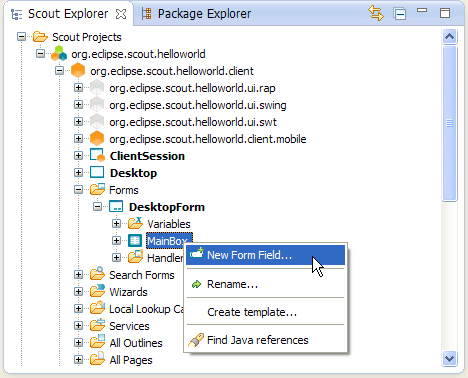
\includegraphics[width=8cm]{sdk_new_field_wizard_menu.png} 
\caption{Using the \menu{New Form Field ...} to start the form field wizard provided by the Scout SDK.}
\figlabel{new_field_context_menu}
\end{figure}

To add any widgets to the desktop form we first need to navigate to the \element{DesktopForm} in the Scout Explorer.
By clicking on the small plus icon on the left hand side of the \element{DesktopForm} this element is expanded and the \element{MainBox} element becomes visible below.
With a click of the right mouse button over the \element{MainBox}, the available context menus are displayed.
To start the form field wizard we select the \menu{New Form Field ...} as shown in \figref{new_field_context_menu}.

\begin{figure}
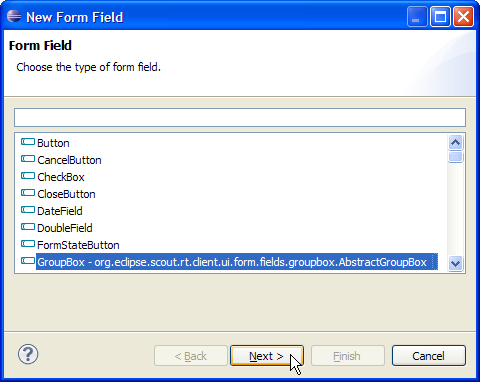
\includegraphics[height=4.5cm]{sdk_new_field_groupbox_1.png} \hspace{8mm}
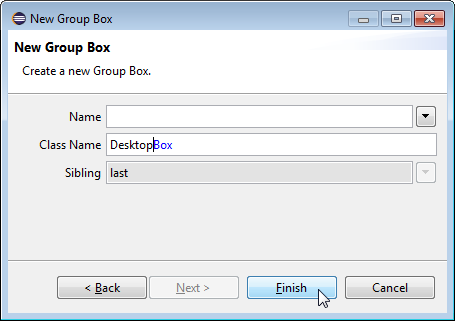
\includegraphics[height=4.5cm]{sdk_new_field_groupbox_2.png}
\caption{Adding the \textit{DesktopBox} field with the Scout SDK form field wizard.}
\index{SDK Wizard!New Form Field}
\figlabel{helloworld_groupboxfield}
\end{figure}

In the first dialog of the form field wizard shown on the left side of \figref{helloworld_groupboxfield}, we choose the form field type.
To select the desired field type, we either select the desired type with the mouse or use the search field to filter the list of available field types.
In the second wizard dialog, we do not provide a label for the group box in the \field{Name}.
As we have only a single group box in the ''Hello World'' desktop form we omit the name and enter 'Desktop' into the \field{Class Name} before we close the wizard with the \button{Finish}.
This step is shown on the right side of \figref{helloworld_groupboxfield}.
The Scout SDK will add the necessary Java code for the \java{DesktopBox} in the background.

\begin{figure}
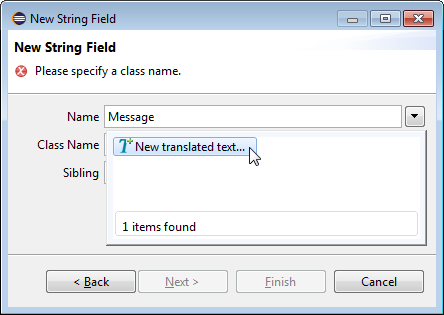
\includegraphics[height=4.2cm]{sdk_new_field_stringfield_1.png} \hspace{8mm}
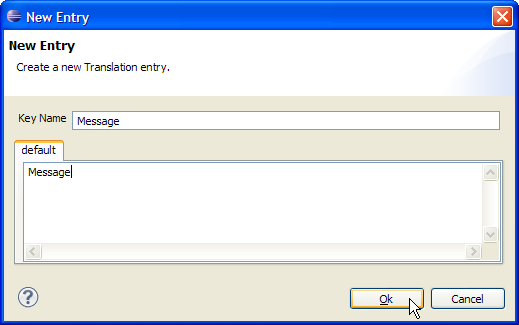
\includegraphics[height=4.2cm]{sdk_new_field_stringfield_2.png}
\caption{Adding a \textit{StringField} and providing a new translation entry.}
\index{SDK Wizard!Add Translation Entry}
\figlabel{helloworld_stringfield}
\end{figure}

To add the text field widget to the group box just created, we navigate to the corresponding \element{DesktopBox} in the Scout Explorer.
For this, we click on the small plus icon on the left hand side of the \element{MainBox} to expand this node and make the \element{DesktopBox} element visible.
On \element{DesktopBox} we again use the \menu{New Form Field ...}.
In the first wizard dialog, we select \element{StringField} using 'st' as a search criteria and click the \button{Next} to open the second wizard dialog.
In the second wizard dialog, we enter 'Message' into the \field{Name}.
As we do not yet have the text 'Message' available in our ''Hello World'' application the wizard prompts the user with the proposal \textsc{New Translated Text ...}.
Selecting the provided option we can add a new text entry as shown in \figref{helloworld_stringfield}.
Once we have provided some initial translation for our message label, we can close the translation dialog with the \button{Ok}.
Finally, we close the form field wizard using the \button{Finish}.

\begin{figure}
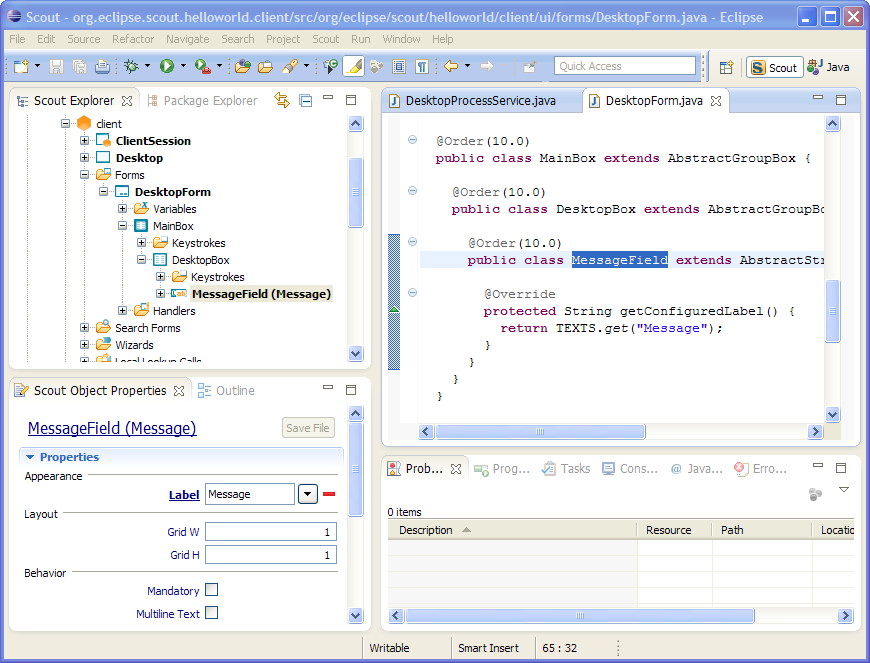
\includegraphics[width=15cm]{sdk_helloworld_messagefield.png}
\caption{Scout SDK showing the \it{MessageField}}
\figlabel{helloworld_messagefield}
\end{figure}

By expanding the \element{DesktopBox} element in the Scout Explorer, the new message field becomes visible. 
A double click on the message field element then loads the corresponding Java code into an Editor as shown in \figref{helloworld_messagefield}.
If you are following this tutorial with your own Eclipse Scout installation compare your status with this screenshot.
Make sure that the project structure in the Scout Explorer looks as shown in \figref{helloworld_messagefield} and a double click to the \element{MessageField} both loads the corresponding Java code and displays the message field's properties in the Scout Object Properties.

Having verified your status of the ''Hello World'' application you can start the application as described in \secref{run_initial}.
The client applications will then display your message widget.
However, the text widget is still empty, as we did not yet load any initial content into it.
This is the topic of the next section where we continue the tutorial with the server part.

% =========================================================================== %
% EOF TeX input file
% =========================================================================== %
